\documentclass[11pt,a4paper]{article}
\usepackage[utf8]{inputenc}
\usepackage[margin=0.8in]{geometry}
\usepackage{tikz}
\usetikzlibrary{shapes.geometric, arrows, positioning, calc, fit, backgrounds}
\usepackage{xcolor}
\usepackage{hyperref}
\usepackage{listings}
\usepackage{graphicx}
\usepackage{tcolorbox}
\usepackage{enumitem}
\usepackage{tabularx}
\usepackage{booktabs}

% Colors
\definecolor{brandblue}{RGB}{33, 150, 243}
\definecolor{brandgreen}{RGB}{76, 175, 80}
\definecolor{brandorange}{RGB}{255, 152, 0}
\definecolor{brandpurple}{RGB}{156, 39, 176}

% TikZ Styles
\tikzstyle{process} = [rectangle, rounded corners, minimum width=3cm, minimum height=1cm, text centered, draw=black, fill=brandblue!20, align=center]
\tikzstyle{decision} = [diamond, minimum width=2.5cm, minimum height=1cm, text centered, draw=black, fill=brandorange!30, aspect=2.5, font=\small, align=center]
\tikzstyle{sensor} = [ellipse, minimum width=2.5cm, minimum height=0.8cm, text centered, draw=black, fill=brandgreen!20, font=\small\bfseries, align=center]
\tikzstyle{action} = [rectangle, minimum width=2.5cm, minimum height=0.8cm, text centered, draw=black, fill=brandpurple!20, font=\small, align=center]
\tikzstyle{arrow} = [thick,->,>=stealth]

\title{\textbf{Control Award Submission}\\Team Portfolio Summary}
\author{Quanta FTC Team}
\date{2026 Season}

\begin{document}

\maketitle

% ============================================================================
% SECTION 1: SYSTEM OVERVIEW (Required 1A & 1C)
% ============================================================================
\section{Control System Overview}

\begin{tcolorbox}[colback=white, colframe=black, title=\textbf{Portfolio Description}]
The Quanta Robot uses a distributed control architecture managed by the REV Control Hub. The system integrates three primary sensor modalities (Inertial, Vision, and Color) to drive automated actions in both TeleOp and Autonomous modes. 

\textbf{Key Innovation:} The integration of Dead Wheel Odometry (`par0`, `par1`, `perp`) allows for "Field-Centric" corrective steering during autonomous intake cycles, solving the problem of mechanical drift caused by uneven friction.
\end{tcolorbox}

\begin{center}
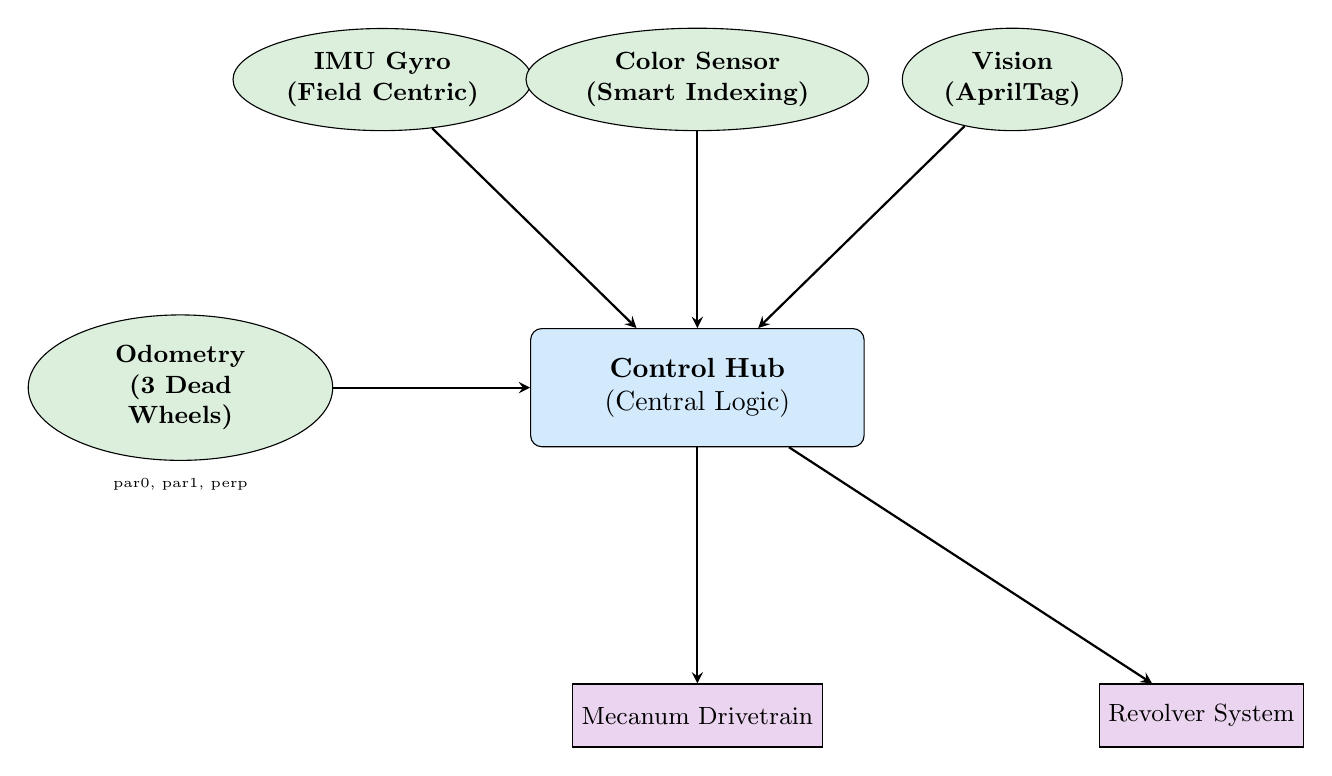
\begin{tikzpicture}[node distance=2.5cm, auto]
    % Central Controller
    \node (hub) [process, text width=4cm, minimum height=1.5cm] {\textbf{Control Hub}\\(Central Logic)};
    
    % Sensors (Top & Sides) - SPACED OUT WIDER
    \node (imu) [sensor, above=of hub, xshift=-4cm] {\textbf{IMU Gyro}\\(Field Centric)};
    \node (color) [sensor, above=of hub, xshift=0cm] {\textbf{Color Sensor}\\(Smart Indexing)};
    \node (vision) [sensor, above=of hub, xshift=4cm] {\textbf{Vision}\\(AprilTag)};
    
    % Dead Wheels (New)
    \node (odo) [sensor, left=of hub, text width=2.5cm, align=center] {\textbf{Odometry}\\(3 Dead Wheels)};
    
    % Actuators (Bottom)
    \node (drive) [action, below=of hub, yshift=-0.5cm] {Mecanum Drivetrain};
    \node (revolver) [action, right=of drive, xshift=1cm] {Revolver System};
    
    % Arrows
    \draw [arrow] (imu) -- (hub);
    \draw [arrow] (color) -- (hub);
    \draw [arrow] (vision) -- (hub);
    \draw [arrow] (odo) -- (hub);
    \draw [arrow] (hub) -- (drive);
    \draw [arrow] (hub) -- (revolver);
    
    % Labels (Integrated into nodes to prevent overlap)
    \node [below=0.1cm of odo, font=\tiny] {par0, par1, perp};
\end{tikzpicture}
\end{center}

% ============================================================================
% SECTION 2: SENSOR LOGIC & ALGORITHMS
% ============================================================================
\section{Sensor Logic: Color Edge Detection}

\begin{tcolorbox}[colback=white, colframe=black, title=\textbf{Portfolio Description}]
To automate the intake process, we implemented an "Edge Detection" algorithm using the REV Color Sensor V3. Instead of simply checking if a ball is present, the software monitors for the exact moment a ball \textit{enters} the sensor's range (Rising Edge).

\textbf{How It Works:}
\begin{enumerate}
    \item \textbf{Filtering:} We calculate a custom metric: $Distance < 4cm$ AND $(Green > Threshold OR Purple > Threshold)$.
    \item \textbf{State Memory:} The system remembers the previous loop's state. If `Current=Detected` and `Previous=Empty`, we trigger an Index Action.
    \item \textbf{Result:} This allows the driver to drive continuously over a stack of pixels without stopping to toggle the indexer manually. A cooldown timer prevents double-counting.
\end{enumerate}
\end{tcolorbox}

\begin{center}
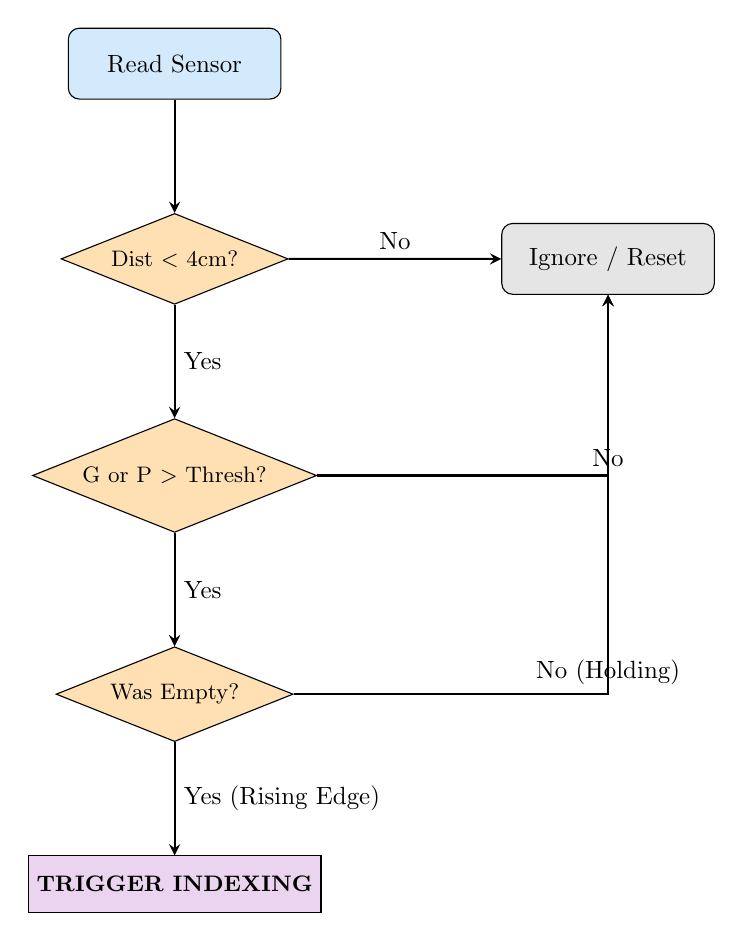
\begin{tikzpicture}[node distance=1.6cm, auto, scale=0.9, transform shape]
    % Vertical spine
    \node (read) [process] {Read Sensor};
    \node (dist) [decision, below=of read] {Dist $<$ 4cm?};
    \node (color) [decision, below=of dist] {G or P $>$ Thresh?};
    \node (edge) [decision, below=of color] {Was Empty?};
    \node (action) [action, below=of edge] {\textbf{TRIGGER INDEXING}};
    
    % Results on right
    \node (ignore) [process, right=3cm of dist, fill=gray!20] {Ignore / Reset};
    
    % Arrows
    \draw [arrow] (read) -- (dist);
    \draw [arrow] (dist) -- node[right] {Yes} (color);
    \draw [arrow] (dist) -- node[above] {No} (ignore);
    
    \draw [arrow] (color) -- node[right] {Yes} (edge);
    \draw [arrow] (color) -| node[above] {No} (ignore);
    
    \draw [arrow] (edge) -- node[right] {Yes (Rising Edge)} (action);
    \draw [arrow] (edge) -| node[above] {No (Holding)} (ignore);
\end{tikzpicture}
\end{center}

\subsection{Localization: 3-Wheel Odometry}
We use a **Three-Dead-Wheel** setup (`par0`, `par1`, `perp`) to track position.
\begin{itemize}
    \item \textbf{Parallel Pods (2):} Track forward/backward movement and heading changes.
    \item \textbf{Perpendicular Pod (1):} Tracks strafe movement (lateral drift).
    \item \textbf{Benefit:} Provides absolute field coordinates $(X, Y, \theta)$ even when drive wheels slip.
\end{itemize}

% ============================================================================
% SECTION 3: INTELLIGENT TELEOP CONTROL
% ============================================================================
\section{Intelligent TeleOp Solutions}

\subsection{Field-Centric Drive Control}

\begin{tcolorbox}[colback=white, colframe=black, title=\textbf{Portfolio Description}]
We solved the challenge of driver disorientation using a Field-Centric Drive algorithm. By continuously initializing the input vector against the robot's IMU Heading, the robot moves relative to the field, not its own chassis.

\textbf{Math Implementation:}
$$ X_{cmd} = X_{joy} \cos(-\theta) - Y_{joy} \sin(-\theta) $$
$$ Y_{cmd} = X_{joy} \sin(-\theta) + Y_{joy} \cos(-\theta) $$
This ensures that pushing the stick "forward" always sends the robot towards the opponent's alliance wall, regardless of whether the robot is spinning or strafing.
\end{tcolorbox}

\subsection{Smart Indexing State Machine}

\begin{tcolorbox}[colback=white, colframe=black, title=\textbf{Portfolio Description}]
The Revolver mechanism controls ball storage. Using a Finite State Machine (FSM), we decoupled the mechanical actions from driver input. The FSM manages the precise timing of spooling up the shooter, checking for ball clearance, and rotating the barrel, ensuring the mechanism never jams due to conflicting commands.
\end{tcolorbox}

\begin{center}
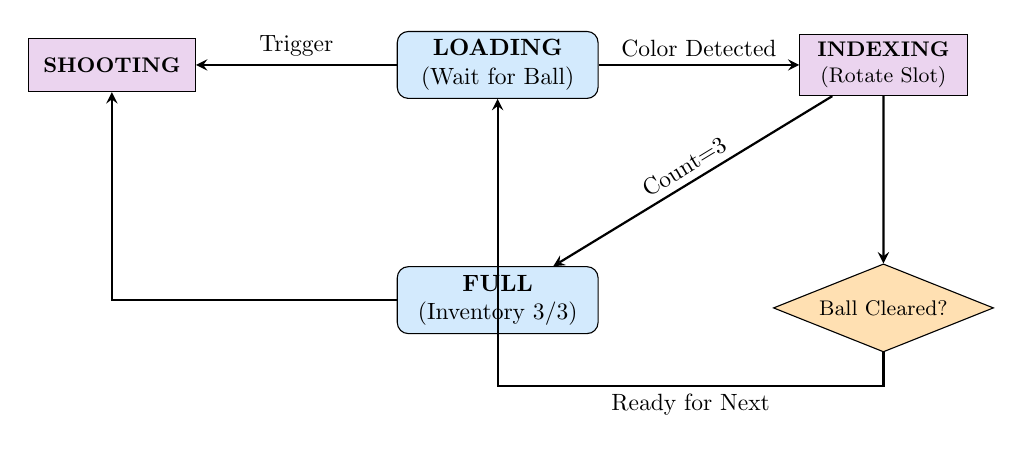
\begin{tikzpicture}[node distance=2.5cm, auto, scale=0.85, transform shape]
    % Nodes spaced out to prevent entanglement
    \node (loading) [process, text width=2.5cm] {\textbf{LOADING}\\(Wait for Ball)};
    
    \node (indexing) [action, right=3cm of loading] {\textbf{INDEXING}\\(Rotate Slot)};
    
    \node (wait) [decision, below=of indexing] {Ball Cleared?};
    
    \node (full) [process, below=of loading] {\textbf{FULL}\\(Inventory 3/3)};
    
    \node (shoot) [action, left=3cm of loading] {\textbf{SHOOTING}};
    
    % Flow Arrows - Curvy to avoid crossing
    \draw [arrow] (loading) -- node[above] {Color Detected} (indexing);
    \draw [arrow] (indexing) -- (wait);
    
    % Return path from Wait -> Loading
    \draw [arrow] (wait.south) -- ++(0,-0.5) -| (loading.south) node[pos=0.25, below] {Ready for Next};
    
    % Shoot Paths
    \draw [arrow] (loading) -- node[above] {Trigger} (shoot);
    \draw [arrow] (full) -| (shoot);
    
    % Full Path
    \draw [arrow] (indexing) -- node[sloped, above] {Count=3} (full);
\end{tikzpicture}
\end{center}

\subsubsection{FSM State Definitions}
Our software tracks the exact status of the mechanism using the following states:

\begin{tabularx}{\textwidth}{|l|X|}
\hline
\textbf{State} & \textbf{System Behavior} \\
\hline
\texttt{LOADING} & Intake is active. Indexer is aligned to an empty slot (0° relative). System monitors color sensor for incoming game elements. \\
\hline
\texttt{INDEXING} & A ball was detected. The indexer motor rotates 60° (96 ticks) to the next slot position. Intake is momentarily paused. \\
\hline
\texttt{WAIT\_CLEAR} & Safety state. The system waits up to 500ms or until the color sensor reads "Empty" to ensure the ball has fully entered the magazine before accepting another. \\
\hline
\texttt{SHOOTING} & Shooter motor spins up to velocity. Kicker servo extends and retracts in a timed sequence to eject the ball. \\
\hline
\texttt{FULL} & All 3 slots are occupied. Intake automatically stops to prevent jamming. Driver must shoot to clear slots. \\
\hline
\end{tabularx}

% ============================================================================
% SECTION 4: AUTONOMOUS RELIABILITY
% ============================================================================
\section{Autonomous Reliability Solutions}

\subsection{Closed-Loop Drift Correction}

\begin{tcolorbox}[colback=white, colframe=black, title=\textbf{Portfolio Description}]
Autonomous intake runs are prone to drift. We implemented a Closed-Loop P-Controller that locks the robot's lateral ($X$) coordinate. During the intake pass, the Odometry pods provide real-time position feedback. Any deviation from the target line generates a counter-strafe command proportional to the error ($Power = K_p \times Error$). This keeps the robot perfectly centered on the sample stack.
\end{tcolorbox}

\subsection{Autonomous Decision Tree}

\begin{center}
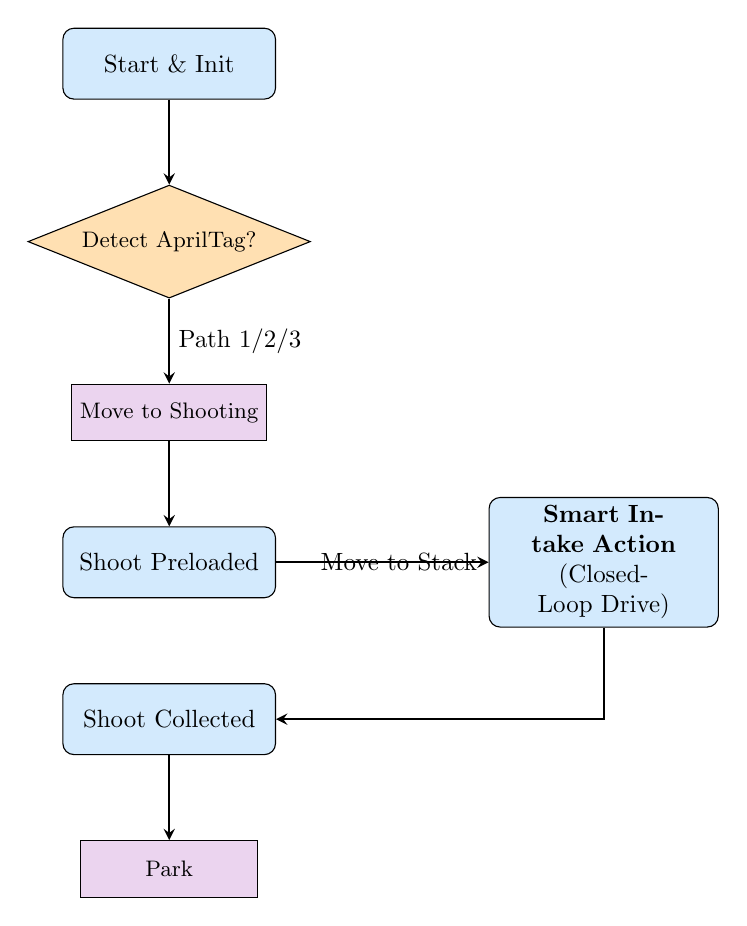
\begin{tikzpicture}[node distance=1.2cm, scale=0.9, transform shape]
    % Vertical Layout for clarity
    \node (start) [process] {Start \& Init};
    \node (vis) [decision, below=of start] {Detect AprilTag?};
    \node (move1) [action, below=of vis] {Move to Shooting};
    \node (shoot1) [process, below=of move1] {Shoot Preloaded};
    
    % Intake Branch
    \node (intake) [process, right=3cm of shoot1, text width=3cm] {\textbf{Smart Intake Action}\\(Closed-Loop Drive)};
    
    % Return
    \node (shoot2) [process, below=of shoot1] {Shoot Collected};
    \node (park) [action, below=of shoot2] {Park};
    
    % Arrows
    \draw [arrow] (start) -- (vis);
    \draw [arrow] (vis) -- node[right] {Path 1/2/3} (move1);
    \draw [arrow] (move1) -- (shoot1);
    
    % Side Loop for Intake
    \draw [arrow] (shoot1.east) -- ++(0.5,0) |- node[pos=0.2, right] {Move to Stack} (intake.west);
    \draw [arrow] (intake.south) |- (shoot2.east);
    
    \draw [arrow] (shoot2) -- (park);
    
\end{tikzpicture}
\end{center}

\section{Summary of Sensors}
\begin{tabularx}{\textwidth}{|l|X|l|}
\hline
\textbf{Sensor} & \textbf{Usage in Algorithm} & \textbf{Component} \\
\hline
\textbf{Control Hub IMU} & Field-centric drive vector transformation & Drivetrain \\
\hline
\textbf{REV Color V3} & Detects ball entry/exit for auto-indexing & Revolver \\
\hline
\textbf{Motor Encoders} & Velocity stabilization \& Odometry & Drive/Shooter \\
\hline
\textbf{Webcam} & AprilTag detection for randomization pattern & Autonomous \\
\hline
\end{tabularx}

\end{document}
